\section{Classification}
\label{sec:classification}
% search / retrieval / classification
Data-driven techniques commonly make assumptions about the size and homogeneity of the input data set. In particular, existing analysis techniques often assume that all models belong to the same class of objects~\cite{Kim:2013:lpt} or scenes~\cite{Fisher:2011:CSR}, and cannot directly scale to entire repository such as the Trimble 3D Warehouse~\cite{warehouse}. Similarly, techniques for data-driven reconstruction of indoor environments assume that the input data set only has furniture models~\cite{Nan:2012:SAC}, while modeling and synthesis interfaces restrict the input data to particular object or scene classes~\cite{Chaudhuri:2011:prabm,Kalogerakis:2012:PMC,Fisher:2012:CSR}.  Thus, as a first step these methods query a 3D model repository to retrieve a subset of relevant models.



There are three most common techniques for specifying the query used in existing shape retrieval systems:
%
\begin{itemize}
\item \textbf{Shape-based} retrieval techniques take an example 3D model as input and output a set of most similar shapes (sometimes accompanied by similarity values). These techniques commonly represent models as high-dimensional feature vectors in shape descriptor space, and use distances in that space to infer model similarity.
\item \textbf{Sketch- or image-based} methods take a 2D depiction as input and search for 3D objects that are similar to the input. These methods often rely on matching geometric features that can be estimated from both 2D and 3D representations, such as silhouette lines.
\item \textbf{Text-based} techniques return results based on shape tags or categories. In most repositories this information is only sparsely associated with 3D data, and thus additional tools are required to enrich repositories of 3D models with relevant annotations.
\end{itemize}

\begin{figure}[b]
\centering
    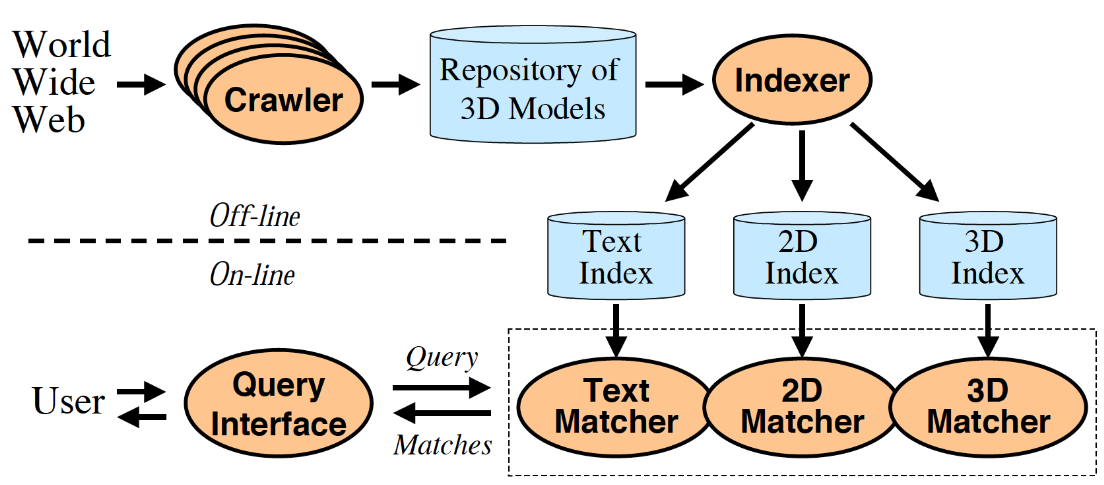
\includegraphics[width=1.0\columnwidth]{fig/search/funk_searchEngine.png}
    \vspace{-.4cm}
    \caption{A search engine framework \cite{Funkhouser:2003:ASE} }
    \vspace{-.6cm}    
    \label{fig:searchEngine}
\end{figure}


While existing search engines commonly support several modalities for a query (e.g. Princeton Search Engine~\cite{Funkhouser:2003:ASE} depicted in Figure \ref{fig:searchEngine} allows all three types of queries), the query matching techniques are often handled by independent algorithms. In the remaining subsections we cover existing methods for each type of user query.

\subsection{Shape-based Retrieval}
\label{sec:shapeBasedSearch}
% motivation
The goal of a shape-based retrieval method is to extract a subset of 3D models from a repository ranked based on their similarity to the input 3D shape. Typically, these techniques index all 3D shapes in a database by computing their shape descriptors in an offline pre-processing stage. In an online stage, the system computes the shape descriptor of a query shape and quickly finds indexed models with similar descriptors.  There are several options for obtaining the query shape. If the user knows a relevant model in the input repository, it could be provided as a query to retrieve a subset of similar models.  Alternatively, the query shape does not have to be a high-quality 3D model, it can be constructed from primitives~\cite{Funkhouser:2004:MBE} or created with a simple modeling tool~\cite{Chaudhuri:2010:ddsc}. For some applications, such as scene reconstruction, the query shape can also be an object acquired with a 3D scanner~\cite{Nan:2012:SAC}.  

% challenges: invariances (as a list?), less than O(n)
Usually shape retrieval techniques use shape descriptors, feature vectors that describe prominent geometric features, to index a database.  A good shape descriptor should yield similar features for similar shapes, and it is expected to be invariant to translations, rotations, and sometimes, scale, since these transformations typically do not change the semantics of a shape.  Most applications also require the shape descriptor to be insensitive to acquisition noise and shape representation, such as different tessellation of meshes or different point sampling. Finally, a repository does not usually contain an exact match for a query, and thus distances between shape descriptors should correspond to perceived differences between models, for example, models that belong to the same class should have small distances. A large number of shape-based retrieval techniques have been developed in recent years~\cite{Tangelder:2008:ASC}. In this document, we overview several shape descriptor techniques that are most commonly used in data-driven methods, grouping them into ones that require models to be aligned to one another, ones that are invariant to alignment, and methods that handle partial data.

%	alignment-dependent: voxels, wavelets, moments, extended Gaussian image, spherical extent function, spherical attribute image, lightfield descriptor
\paragraph*{Alignment-dependent.}
A consistent alignment of shapes automatically provides invariance with respect to translation, rotation, and scale. Once shapes are aligned, one can directly compare how surfaces are distributed in space. Funkhouser et al. \cite{Funkhouser:2003:ASE} describe a shape as a volumetric grid.
% where each cell stores Gaussian of a Euclidean distance to the surface. 
This representation is simple to compute, but it relies on accurate alignment of shapes and leads to relatively big feature vectors. Several techniques represent shapes as spherical functions. For example, Extended Gaussian Image representation~\cite{Horn:1984:EGI} uses a histogram of distribution of surface normals over a sphere. Ankerst et al.~\cite{Ankerst:1999:3dsh} represent 3D models as spherical functions measuring surface area in each direction from the origin. Saupe et al.~\cite{Saupe:2001:MRS} define a spherical function based on the distance to the last point of intersection of the model with the ray. Chen et al.~\cite{Chen:2003:ovsb} render model silhouettes from different viewpoints on a sphere and compare the resulting images.

While alignment-dependent descriptors are effective in retrieving relevant shapes, finding an appropriate alignment for all pairs of shapes is too complex for effective retrieval.  Thus, these methods typically index shapes based on a canonical alignment, which is produced independently for each shape.  Horn et al.~\cite{Horn:1987:cfs,Horn:1988:cfs} suggest that an optimal alignment should minimize the sum of square differences between two ordered point sets, and prove that optimal translation and isotropic scale can be computed for each model, independently of all the other models. The optimal translation aligns center of object's mass, and the scale is set so that the mean variance in point distances to the center of mass is one. Kazhdan et al. \cite{Kazhdan:2004:SMA} define optimal anisotropic scale, and demonstrate that scaling shapes anisotropically improves retrieval results.

Unfortunately, optimal rotation cannot be computed for each model independently, and thus choosing canonical rotations poses a bigger challenge. One possibility is to align principal axes to x-, y-, z-~\cite{Duda:2000:PC}. Alternatively, Podolak et al.~\cite{Podolak:2006:PRST} suggest using principal symmetry axis, which iteratively finds the best symmetry planes, 
%orthogonal to one another, 
where the symmetry plane is scored based on how well the object aligns with itself under reflection around a plane. They also use the intersection of symmetry planes to define a canonical translation. 
%To all of these methods, 
However, finding a canonical alignment is not always reliable and leads to additional computational overhead, which motivates developing alignment-independent methods.

%	alignment-independent: shape histogram, harmonic descriptor, shape distributions, bag of words / bag of features
\noindent \textbf{Alignment-independent}
techniques usually focus on rotation invariance since translation and scale can be normalized independently for each model. One way to achieve rotational invariance is to consider distances between points, since they are not affected by rotation. For example, Ankerst et al.~\cite{Ankerst:1999:3dsh} take histogram of distances to the center of mass, while Osada et al.~\cite{Osada:2002:sd} look at histograms of distances between all pairs of points.  Alternatively, rotation-dependent shape descriptors based on spherical and voxel functions can be converted into rotationally invariant ones. For example, Kazhdan et al.~\cite{Kazhdan:2003:RISH} use spherical harmonics for this purpose. In particular, they describe and compare spherical functions in terms of amount of energy contained at different frequencies. Novotni et al.~\cite{Novotni:2003:3DZD} extend spherical harmonics based descriptors using 3D Zernlike invariants.  In addition to rotation-invariance, several recent works focus on computing features that are invariant to isometric deformations, such as articulation in human poses. One effective example, is a multi-scale Heat Kernel signature, which captures the amount of heat coming back to point at different time scales~\cite{Sun:2009:CPI}. These features can be used in combination with a bag-of-words approach to produce histogram-based shape descriptors~\cite{Bronstein:2011:SGGW}.

Most shape descriptors listed above assume that the entire 3D model is available as input. This would not work well if only part of a query model is observed, or if a model is a part of a bigger scene (e.g.~\cite{Nan:2012:SAC}).

% spin images, priority-driven
\noindent \textbf{Partial} retrieval methods are designed to handle cases when only some regions of query and retrieved models are similar.  If the query is a scene containing a model of interest, one can segment the model or region from the scene in a pre-processing step and use global shape descriptors~\cite{Golovinskiy:2009:SBR3D}. In more challenging cases, if a query and a database shape are only partially similar, one can index models based on local shape descriptors, like the ones mentioned in Section \ref{sec:overview}, extracted at points of interest, then match subsets of these points~\cite{Funkhouser:2006:pm3d}.
%Local shape descriptors are typically similar to global descriptors computed at different radii around a feature point. 
%Another commonly used local shape descriptor is spin images proposed by Johnson~\cite{Johnson:1997:siar}. They describe a point of interest by projecting points in its neighborhood on a 2D image parameterized by distances to a tangent plane and distances to a line orthogonal to the tangent plane.

%todo: more on spin images

%\noindent \textbf{Structure-aware}
% todo -- should it be included?
%Several retrieval techniques have been proposed that take advantage of shape structure. This is especially useful in understanding in-class structural variability. Previous methods took advantage of skeletal structure~\cite{Sundar:2004:sksm},
%part structure~\cite{}, reflective~\cite{Kazhdan:2003:ARSD,Podolak:2006:PRST} and other types of  symmetry~\cite{Kazhdan:2004:SD3D}.
%% graph-based similarity
%%skeleton-based similarity


\subsection{Sketch- or image- based Retrieval}
% todo: figure from Eitz paper
%\cite{Xu:2013:SSC} % context can be used for scenes ??
Generating or finding query models might require substantial effort, thus several interfaces offer the option of sketching the query~\cite{Funkhouser:2003:ASE}. Typically, they assume that the contour of a model from a particular viewpoint should roughly coincide with a sketch~\cite{Lee:2008:sbsc}. In addition to contours, Eitz et al.~\cite{Eitz:2012:sbsr} generate canny lines and suggestive contours and use a database of human sketches to find discriminative line features for shape retrieval.  In addition to sketches one can query a system with a real-world image. If image depicts a relatively isolated object one can extract silhouette or other feature lines and use the same techniques as in sketch-based retrieval~\cite{Xu:2011:PMO}.

%\cite{Xiang:2014:BPA} % silvio: beyond pascal
%\cite{Xiang:2014:mmot} % silvio: aspect parts
%\cite{Held:2014:cc3s} % silvio: rss paper, shape, color, motion

\subsection{Text-based Retrieval and Classification}
\label{sec:classText}
Despite recent advances in shape- and sketch-based retrieval users still heavily rely on text to search for models. For example, a user study by Min et al.~\cite{Min:2003:EEW} reports that 67\% of users prefer to use text to perform search. Among non-academic work, one of the biggest shape repositories, Trimble 3D Warehouse~\cite{warehouse}, only allows text-based search. Although text-based search is a popular tool, unfortunately, many shapes do not have clean annotations~\cite{Min:2004:ACO} and thus become unretrievable. This motivates developing automatic algorithms to infer text associated with models. Existing work focuses on establishing class memberships for an entire shape (e.g. this shape is a dog), as well as inferring finer-scale attributes (e.g. this dog has a tail). Typically, these algorithms assume that some example shapes have been labeled, and propagate the labels to unannotated shapes.

\noindent \textbf{Classification} methods assign a class membership for unlabeled shapes. Given a database of annotated models, one can use an unlabeled shape as a query and transfer a label from the most similar retrieved model. Thus, shape-based retrieval methods are often used for shape classification. In fact, shape retrieval benchmarks evaluate the quality of a retrieval algorithm by computing the fraction of retrieved results that belong to the same class as the query~\cite{Shilane:2004:TPS}. Some techniques also use standard machine learning tools coupled with shape descriptors to classify 3D shapes~\cite{Frome:2004:rord,Golovinskiy:2009:SBR3D}. Barutcuoglu et al.~\cite{Barutcuoglu:2006:hscu} demonstrate that Bayesian aggregation can be used to improve classification of shapes that are a part of a hierarchical ontology of objects.

% todo: figure for chaudhuri, for huang
\begin{figure}[bt]
\centering
    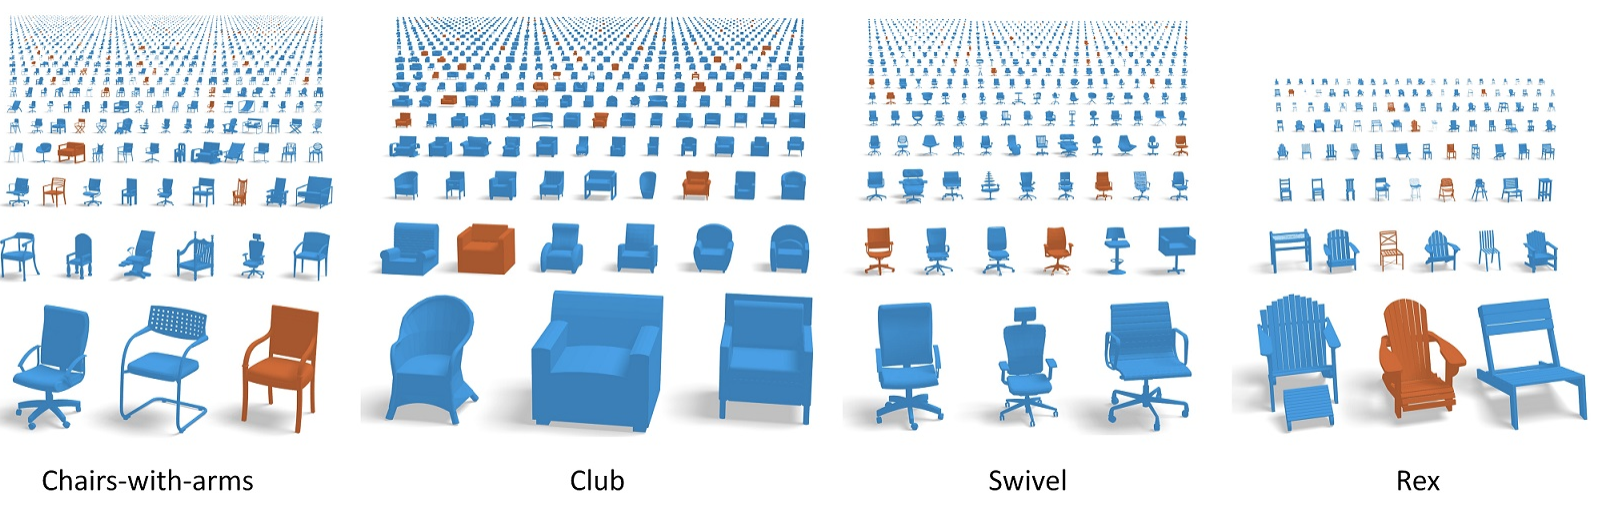
\includegraphics[width=1.0\columnwidth]{fig/search/huang_siga13_fine.png}
   %\vspace{-.6cm}
    \caption{
    Fine-grained classification of 3D models \cite{Huang:2013:FSL}, where text labels are propagated from brown to blue models. }
    \label{fig:fine-grained}
\end{figure}


\noindent \textbf{Tag attributes} often capture fine-scale attributes of shapes that belong to the same class. These attributes can include presence or absence of particular parts, object style, or comparative adjectives. Huang et al.~\cite{Huang:2013:FSL} developed a framework for propagating these attributes in a collection of partially annotated 3D models. For example, only brown models in Figure \ref{fig:fine-grained} were labeled, and blue models were annotated automatically. To achieve automatic labeling, they start by co-aligning all models to a canonical domain, and generate a voxel grid around the co-aligned models. For each voxel they compute local shape features, such as spin images, for each shape. Then, they learn a distance metric that best discriminates between different tags. All shapes are finally embedded in a weighted feature space where nearest neighbors are connected in a graph. A graph cut clustering is used to assign tags to unlabeled shapes.

\begin{figure}[tb]
\centering
    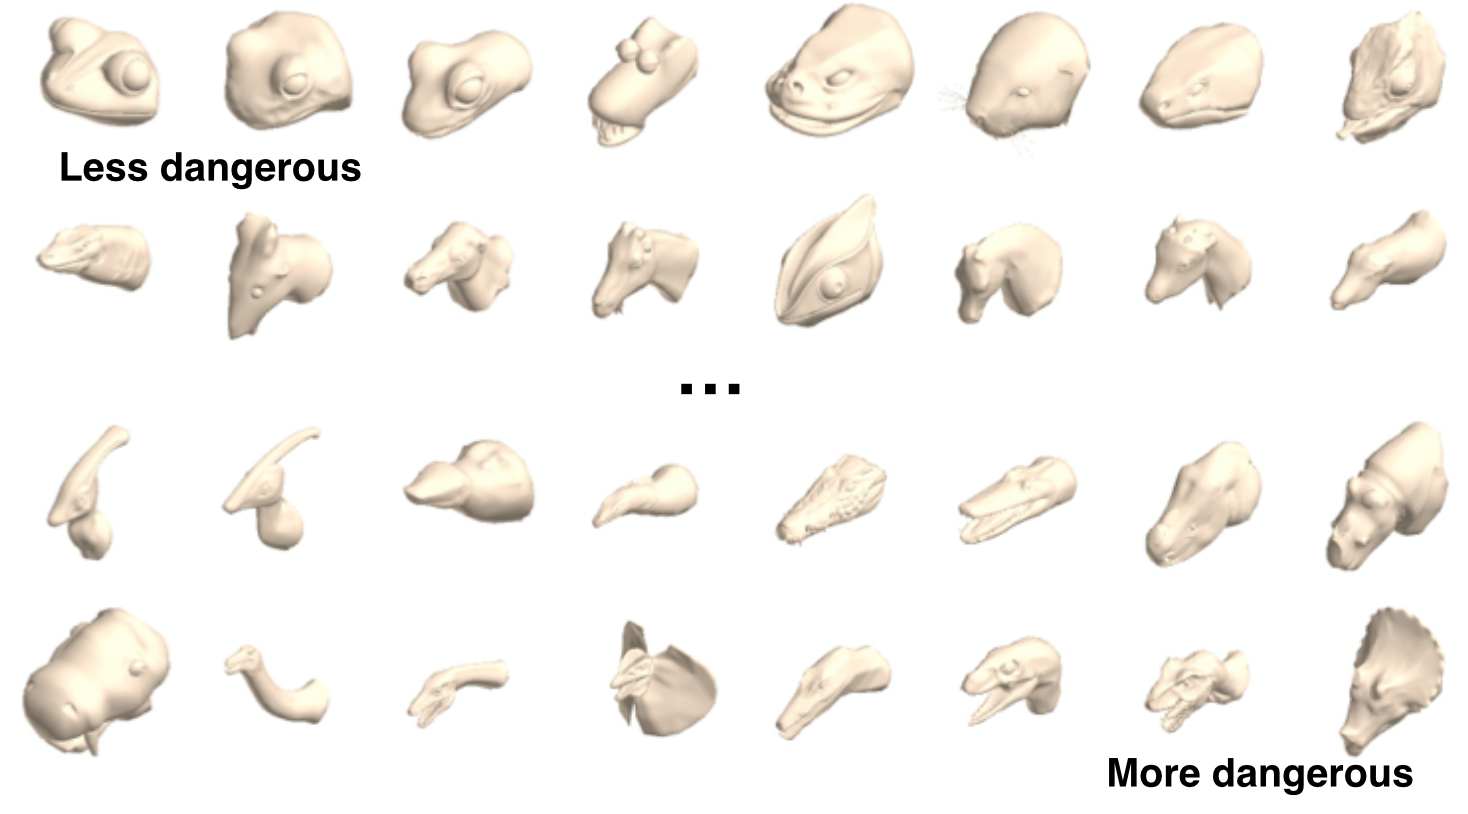
\includegraphics[width=1.0\columnwidth]{fig/search/chaudhuri_uist13_attr.png}
    %\vspace{-.6cm}
    \caption{
    Ranking of parts with respect to ``dangerous'' attribute (image from \cite{Chaudhuri:2013:ACC}) }
    \label{fig:attribit}
\end{figure}


While above method works well for discrete tags, it does not capture more continuous relations, such as animal A is more dangerous than animal B.  Chaudhuri et al.~\cite{Chaudhuri:2013:ACC} focus on estimating ranking based on comparative adjectives. They ask people to compare pairs of shape parts with respect to different adjectives, and use a Support Vector Machine ranking method to predict attribute strengths from shape features for novel shapes (Figure \ref{fig:attribit}).

%\subsection{Discussion of retrieval techniques}
% limitations
While the techniques described above are suitable for retrieving related models, most of the described method are not designed to understand intra-class variations. Usually a more involved structural analysis is necessary to understand higher-level semantic properties of shapes. Even for inferring tag attributes existing works relies on shape matching~\cite{Huang:2013:FSL} or shape segmentation~\cite{Chaudhuri:2013:ACC}. The following two sections will focus on inferring these higher-level structural properties in collections of shapes.

% structure-aware descriptors
